\documentclass{article}
\usepackage{qilin}
\hfuzz=1000pt 
\newcommand{\bff}[1]{\mathbf{#1}}
\newcommand{\image}[1]{\mathrm{im}\,#1}
\newcommand{\spann}[1]{\mathrm{span}\{#1\}}
\newcommand{\spannn}[1]{\mathrm{span}\,#1}
\newcommand{\floor}[1]{\mathrm{floor}\left(#1\right)}
\usepackage{neuralnetwork}

% \newcommand{\dim}[1]{\mathrm{dim}\,#1}
\usepackage{blkarray}
\usepackage{pythonhighlight}
\tikzset{
  heap/.style={
    every node/.style={circle,fill=black!25,minimum size=20pt,inner sep=2pt},
    tree/.style={
        draw=red!50,
        shape=isosceles triangle,
        fill=red!50,
        minimum height=30pt,
        minimum width=20pt,
        shape border rotate=90,
        inner sep=2pt,
        yshift = -5pt,
    },
    big tree/.style={
        draw=red!50,
        shape=isosceles triangle,
        fill=red!50,
        minimum height=60pt,
        minimum width=25pt,
        isosceles triangle stretches,
        shape border rotate=90,
        inner sep=2pt,
        yshift = -30pt,
    },
    level 1/.style={sibling distance=30mm},
    level 2/.style={sibling distance=10mm}
  }
}
\newcommand{\node}[1]{
    \begin{tikzpicture}[scale=0.5, baseline=-2mm]
        \tikzstyle{vertex}=[circle,fill=black!25,outer xsep=-10pt]
        \node[vertex] (N) at (0,-0.1) {#1};
    \end{tikzpicture}
}
\newcommand{\tree}[1]{
    \begin{tikzpicture}[scale=0.1, baseline=-2mm]
        \tikzstyle{vertex}=[
            draw=red!50,
            shape=isosceles triangle,
            fill=red!50,
            minimum height=20pt,
            minimum width=15pt,
            shape border rotate=90,
            inner sep=0pt,
            yshift = -3pt
        ]
        \node[vertex] (N) at (0,-0.1) {#1};
    \end{tikzpicture}
}



\title{\textbf{ESC190 Exam Review:} \\ Data Structures and Algorithms}
\author{QiLin Xue}
\lhead{ESC190}
\rhead{QiLin Xue}

\begin{document}
    \maketitle
    \tableofcontents
    \newpage
    % \section{Preface}
    % In this document, I will primarily use \textit{Python} to illustrate the theory behind the different data structures. Since some portions of the midterm will be written in \textit{C}, I have done my best to write my code such that it can be easily adaptable 
    \section{Data Structures}
    \subsection{Linked List}
    A linked list uses \textit{pointers} to link from one object to another. In $C$, this is a practical way of describing lists that allow for inserting and deleting new entries, which we will call nodes. This is because we do not need to allocate this memory beforehand, which is especially handy if we do not know how large our list will be. You should be familiar with how to implement the following functions in $C$ related to linked lists:
    \begin{itemize}
        \item Creating a linked list
        \item Deleting the linked list
        \item Appending a node at a certain position
        \item Deleting a node at a certain position
        \item Finding a node which has a specific value
        \item Looking to see if there is a loop
    \end{itemize}
    The last node of a linked list should always point to the $\verb#null#$ pointer.
    \label{linked list}
    \subsection{Stacks}
    Stacks retrieve information in a \textit{last} in, \textit{first} out order.
    \inputpython{stack.py}{1}{100}

    \subsection{Queues}
    Queues retrieve information in a \textit{first} in, \textit{first} out order
    \inputpython{queue.py}{1}{100}

    \subsection{Priority Queues}
    Priority queues are similar to regular queues, except all entries are flagged with a specific weight. There are three primary operations:
    \begin{itemize}
        \item Inserting an entry and its weight into a priority queue.
        \item Find the entry with the minimum / maximum weight
        \item Retrieve the entry with the minimum / maximum weight
    \end{itemize}
    \subsection{Heaps}
    A heap is used to implement a priority queue. It takes the form of a binary tree, which can be read as a list. The only other condition for a heap is that the parent is smaller than both children. For example, $[1, 3, 9, 7, 5]$ refers to the following tree:
    \begin{center}
        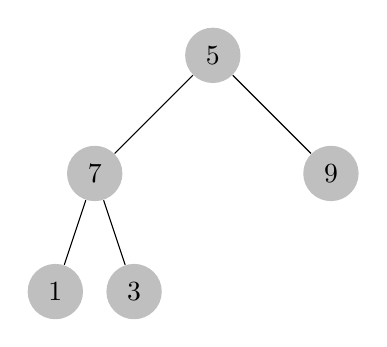
\begin{tikzpicture}[heap]
            \node {5}
            child{node{7}
              child{node{1}} child{node{3}}}
            child{node{9}}
            ;
          \end{tikzpicture}
    \end{center}
    We can denote nodes that do not have any children as \textbf{leaves}. To turn this into a heap, we start at the topmost parent, and we see if it is smaller than both its children. Since this is true, we move on to its first child \node{7}, which is bigger than both its children. As a result, we swap it with the smallest of its two children \node{1}, and we start over the same process, going back to \node{5}. Both BFS (see \ref{bfs}) and DFS (see \ref{dfs}) can be used. The following illustrates the step by step tree diagram representations of the heap.
    \begin{center}
        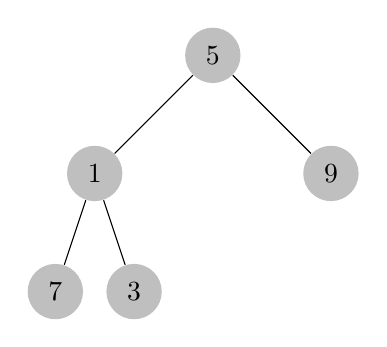
\begin{tikzpicture}[heap]
            \node {5}
            child{node{1}
              child{node{7}} child{node{3}}}
            child{node{9}}
            ;
          \end{tikzpicture}
          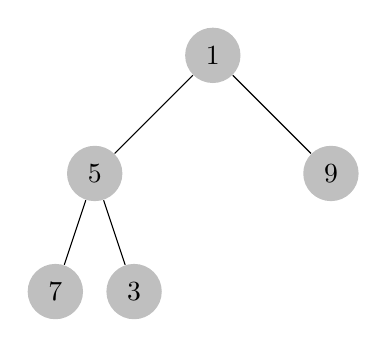
\begin{tikzpicture}[heap]
            \node {1}
            child{node{5}
              child{node{7}} child{node{3}}}
            child{node{9}}
            ;
          \end{tikzpicture}
          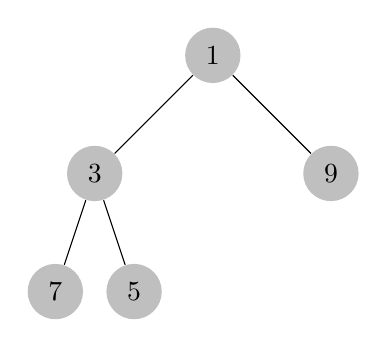
\begin{tikzpicture}[heap]
            \node {1}
            child{node{3}
              child{node{7}} child{node{5}}}
            child{node{9}}
            ;
          \end{tikzpicture}
    \end{center}
    We can use Python to verify this:
    \inputpython{heap.py}{1}{4}
    To add an element, we first place it at the next position of the tree (or the last position of the heap). We then ``percolate'' it up, comparing it with the parent until it is in the right spot. For example, suppose we wish to add \node{4}. Then the process will look like:
    \begin{center}
        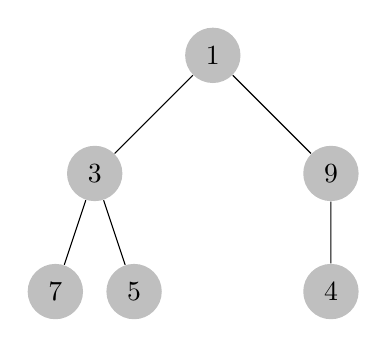
\begin{tikzpicture}[heap]
            \node {1}
            child{node{3}
              child{node{7}} child{node{5}}}
            child{node{9}child{node{4}}}
            ;
          \end{tikzpicture}
          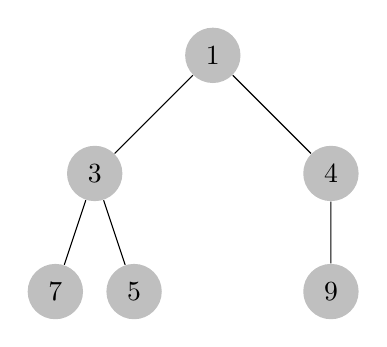
\begin{tikzpicture}[heap]
            \node {1}
            child{node{3}
              child{node{7}} child{node{5}}}
            child{node{4}child{node{9}}}
            ;
          \end{tikzpicture}
    \end{center}
    In Python, we can represent this as:
    \inputpython{heap.py}{6}{7}
    Since this is a priority queue, when we remove an element, we remove the smallest element which will always be at the very top. We can accomplish this by swapping this with the last element, and bubbling that element down. For example, suppose we wish to remove the smallest element \node{1}:
    \begin{center}
          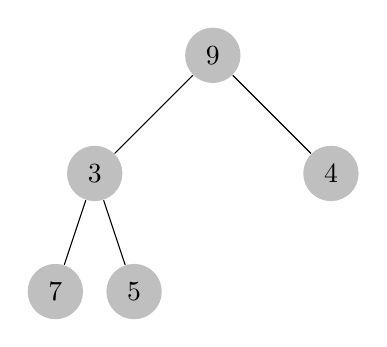
\begin{tikzpicture}[heap]
            \node {9}
            child{node{3}
              child{node{7}} child{node{5}}}
            child{node{4}}
            ;
          \end{tikzpicture}
          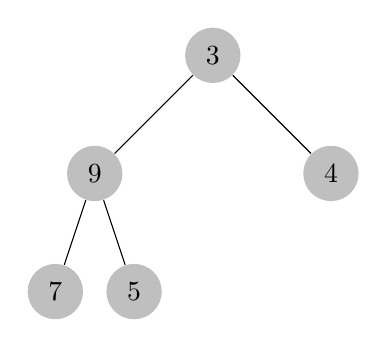
\begin{tikzpicture}[heap]
            \node {3}
            child{node{9}
              child{node{7}} child{node{5}}}
            child{node{4}}
            ;
          \end{tikzpicture}
          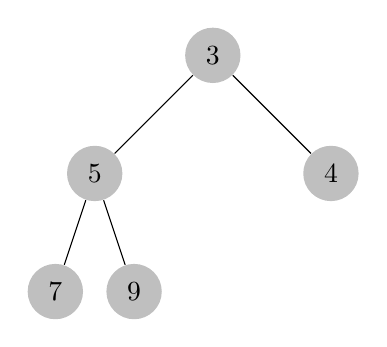
\begin{tikzpicture}[heap]
            \node {3}
            child{node{5}
              child{node{7}} child{node{9}}}
            child{node{4}}
            ;
          \end{tikzpicture}
    \end{center}
    Using Python, we have:
    \inputpython{heap.py}{9}{10}
    \subsubsection{Manual Implementation}
    Using this Python module makes working with heaps trivial and allows us to easily use a list. However, it is also possible to implement this manually with the following mathematical operations. Let the index of an element be $i$. Then:
    \begin{itemize}
        \item Index of parent: $\floor{\frac{i}{2}}$
        \item Index of left child: $2i$
        \item Index of right child: $2i+1$
    \end{itemize}
    For convention, let $i=0$ correspond to a $\verb#Null#$ element. 
    The manual implementation of heapify using Python is shown below:
    \inputpython{manual_heapify.py}{1}{100}
    \subsubsection{Runtime}
    If there are $n$ entries, then we will percolate downwards on average $n/2$ times. The time complexity of percolating downwards is $\mathcal{O}(\log n)$, so the time complexity of heaipfying a list is $\mathcal{O}(n\log n)$.

    However, it is possible to gain a better upper bound. We know that there are at least $n/2$ leaves in the heap. There are $n/4$ nodes at height $1$ (let the bottommost layer be $h=0$). There are $n/8$ nodes at height $2$, and so forth. Therefore at a height $h$, we perform:
    \begin{equation*}
        N_h \propto h \cdot \frac{n}{2^{h+1}}
    \end{equation*}
    operations such that the total number of operations is proportional to:
    \begin{equation*}
        N = \sum_{h=1}^{\log_2{n}} h \cdot \frac{n}{2^{h+1}} \propto h
    \end{equation*}
    so the total runtime is $\mathcal{O}(n)$.
    \subsubsection{Heapsort}
    We can implement a heap to sort a list with a time complexity of $\mathcal{O}(n\log n)$. We perform the following steps:
    \begin{enumerate}
        \item Create a heap from the list.
        \item Extract the minimum a total of $n$ times, and placing the elements into a list in the original order.
    \end{enumerate}
    \section{Graph Theory}
    \subsection{Background}
    \begin{itemize}
        \item We can represent a graph as $G=(V, E)$ where $V$ is the set of nodes $V=\{v_1,v_2, \dots v_n\}$ and $E$ is the set of edges $E=\{e_1, e_2, \dots, e_m\}$. 
        \item Each edge can be written as $e_k = (v_i, v_j)$.
        \item Directed graphs, or \textbf{digraphs} have edges with directions associated with them.
        \item Weighted graphs have a weight associated with each edge.
        \item Vertex $v_1$ is \textbf{adjacent} to vertex $v_2$ if an edge connects them.
        \item A \textit{path} is a sequence of vertices in which each vertex is adjacent to the next one. The length of the path is the number of edges in it.
        \item A cycle in a path is a sequence $(v_1, \dots, v_n)$ such that $(v_i, v_{i+1}) \in E$ and $(v_n, v_1) \in E$.
        \item A graph with no cycles is known as \textbf{acyclic}.
        \item A directed graph which is acyclic is known as a \textbf{DAG}.
        \item A \textbf{simple path} and a \textbf{simple cycle} has no repeated vertices.
        \item Two vertices are \textbf{connected} if there is a path between them.
        \item A subset of vertices is a connected component of a graph $G$ if each pair of vertices in the subset are connected.
        \item The \textbf{degree} of vertex $v$ is the number of edges associated with $v$.
    \end{itemize}
    \subsection{Representing Graphs}
    Suppose we take the following graph:
    \begin{center}
        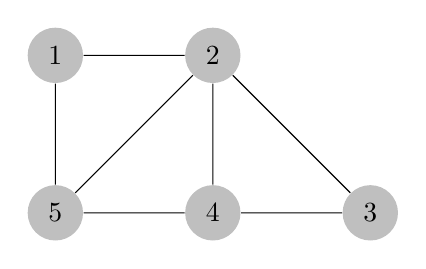
\begin{tikzpicture}[x=2cm, y=2cm]
            \tikzstyle{vertex}=[circle,fill=black!25,minimum size=20pt,inner sep=2pt]
            \node[vertex] (G_1) at (0,1)  {1};
            \node[vertex] (G_2) at (1,1)  {2};
            \node[vertex] (G_3) at (2,0)  {3};
            \node[vertex] (G_4) at (1,0)  {4};
            \node[vertex] (G_5) at (0,0)  {5};
            
            \draw (G_1) -- (G_2) -- (G_3) -- (G_4) -- (G_5) -- (G_1) -- cycle;
            \draw (G_5) -- (G_2) -- (G_4) -- cycle;
        \end{tikzpicture}
    \end{center}
    \subsubsection{Adjacency Matrix}
    For the above graph, the adjacency matrix will look like:
    \begin{equation*}
        A = \begin{blockarray}{cccccc}
            & 1 & 2 & 3 & 4 & 5 \\
            \begin{block}{c[ccccc]}
                1&0&1&0&0&1 \\ 
                2&1&0&1&1&1 \\ 
                3&0&1&0&1&0 \\ 
                4&0&1&1&0&1 \\
                5&1&1&0&1&0 \\
            \end{block}
            \end{blockarray}
    \end{equation*}
    To look up if \node{1} is connected to \node{2}, we just need to look up $\verb#A[2,1] = A[1,2]#$ (or in terms of Python notation, $\verb#A[2][1]#$ or $\verb#A[1][2]#$). Note that adjacency matrices are symmetric (e.g. $A^T = A$) for undirected graphs. It has the following complexities:
    \begin{itemize}
        \item Edge lookup: $\mathcal{O}(1)$
        \item Finding all vertices adjacent to vertex: $\mathcal{O}(|V|)$
        \item Space complexity: $\mathcal{O}(|V|^2)$
    \end{itemize}

    \subsubsection{Adjacency List}
    An adjacency list uses linked lists (see sec. \ref{linked list}) to represent the graph:
    \begin{center}
        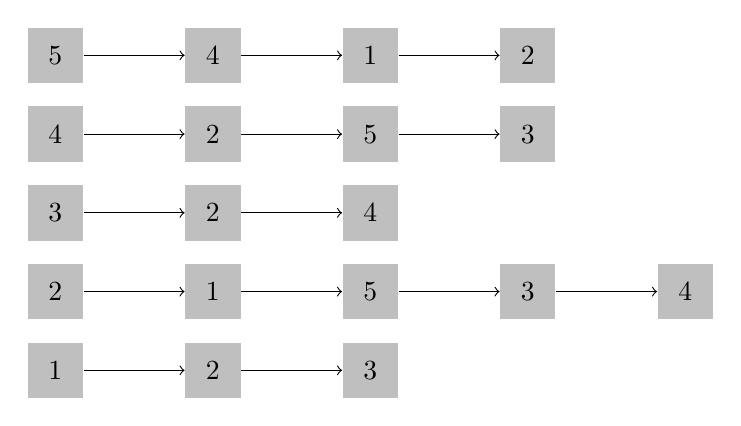
\begin{tikzpicture}[x=2cm, y=2cm]
            \tikzstyle{vertex}=[fill=black!25,minimum size=20pt,inner sep=2pt]
            \node[vertex] (A1) at (0,0)  {1};
            \node[vertex] (A2) at (1,0)  {2};
            \node[vertex] (A3) at (2,0)  {3};

            \node[vertex] (B1) at (0,0.5)  {2};
            \node[vertex] (B2) at (1,0.5)  {1};
            \node[vertex] (B3) at (2,0.5)  {5};
            \node[vertex] (B4) at (3,0.5)  {3};
            \node[vertex] (B5) at (4,0.5)  {4};
            
            \node[vertex] (C1) at (0,1)  {3};
            \node[vertex] (C2) at (1,1)  {2};
            \node[vertex] (C3) at (2,1)  {4};

            \node[vertex] (D1) at (0,1.5)  {4};
            \node[vertex] (D2) at (1,1.5)  {2};
            \node[vertex] (D3) at (2,1.5)  {5};
            \node[vertex] (D4) at (3,1.5)  {3};

            \node[vertex] (E1) at (0,2)  {5};
            \node[vertex] (E2) at (1,2)  {4};
            \node[vertex] (E3) at (2,2)  {1};
            \node[vertex] (E4) at (3,2)  {2};

            \draw[->] (A1) edge (A2) (A2) edge (A3);
            \draw[->] (B1) edge (B2) (B2) edge (B3) (B3) edge (B4) (B4) edge (B5);
            \draw[->] (C1) edge (C2) (C2) edge (C3);
            \draw[->] (D1) edge (D2) (D2) edge (D3) (D3) edge (D4);
            \draw[->] (E1) edge (E2) (E2) edge (E3) (E3) edge (E4);

        \end{tikzpicture}
    \end{center}
    This has the following complexities:
    \begin{itemize}
        \item Edge lookup: $\mathcal{O}(d)$ where $d$ is the maximum degree in the graph
        \item Finding all vertices adjacent to vertex: $\mathcal{O}(d)$
        \item Space complexity: $\mathcal{O}(|V|+|E|)$
    \end{itemize}
    \subsection{Traversal Algorithms}
    We will apply both DFS and BFS to traverse the following graph:
    \begin{center}
        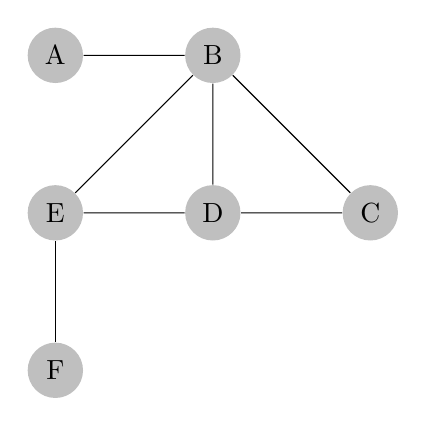
\begin{tikzpicture}[x=2cm, y=2cm]
            \tikzstyle{vertex}=[circle,fill=black!25,minimum size=20pt,inner sep=2pt]
            \node[vertex] (G_1) at (0,1)  {A};
            \node[vertex] (G_2) at (1,1)  {B};
            \node[vertex] (G_3) at (2,0)  {C};
            \node[vertex] (G_4) at (1,0)  {D};
            \node[vertex] (G_5) at (0,0)  {E};
            \node[vertex] (G_6) at (0,-1)  {F};

            \draw (G_1) -- (G_2) -- (G_3) -- (G_4) -- (G_5) -- cycle;
            \draw (G_5) -- (G_2) -- (G_4) -- cycle;
            \draw (G_5) -- (G_6) -- cycle;
        \end{tikzpicture}
    \end{center}
    We can represent this graph using Python:
    \inputpython{search.py}{1}{24}
    \subsubsection{Breadth First Search}
    To implement BFS, we use a queue. Suppose we start our search from $C$. We would explore the nodes in the following order:
    \begin{equation*}
        C \to B \to D \to A \to E \to F
    \end{equation*}
    We visit nodes in the order of the queue and every time a node is visited, the unvisited neighbours of that node is added to the back of the queue. See this Python implementation:
    \inputpython{search.py}{26}{37}
    \label{bfs}
    \subsubsection{Depth First Search}
    \label{dfs}
    In a depth first search, we make use of a stack instead. Nodes are visited in the order of the stack, and every time a node is visited, its unvisited neighbours are added to the stack. Starting from $C$, the nodes are explored in the following order:
    \begin{equation*}
        C \to D \to E \to F \to B \to A
    \end{equation*}
    which can be shown using Python:
    \inputpython{search.py}{53}{64}
    Alternatively, we can use recursion:
    \inputpython{search.py}{69}{78}
    Note that the nodes are traversed in a different order, since the implementation is slightly different. However, it is still DFS.
    \section{Shortest Path Algorithm}
    The general problem here is that we want to find the shortest path between two points through a graph. To do this, we can create a weighted graph, such as below:
    \begin{center}
        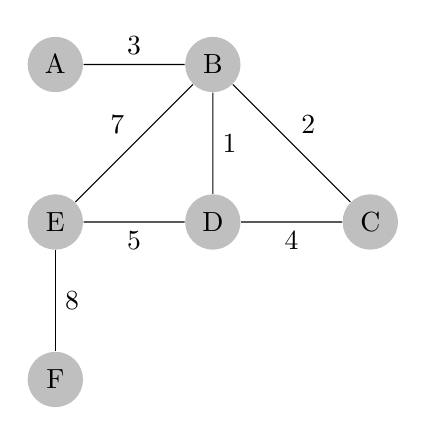
\begin{tikzpicture}[x=2cm, y=2cm]
            \tikzstyle{vertex}=[circle,fill=black!25,minimum size=20pt,inner sep=2pt]
            \node[vertex] (G_1) at (0,1)  {A};
            \node[vertex] (G_2) at (1,1)  {B};
            \node[vertex] (G_3) at (2,0)  {C};
            \node[vertex] (G_4) at (1,0)  {D};
            \node[vertex] (G_5) at (0,0)  {E};
            \node[vertex] (G_6) at (0,-1)  {F};

            \draw (G_1) -- (G_2) node[midway,above] {$3$} -- (G_3) node[midway,above right] {$2$}-- (G_4) node[midway,below] {$4$} -- (G_5) node[midway,below] {$5$} -- cycle;
            \draw (G_5) -- (G_2) node[midway,above left] {$7$} -- (G_4) node[midway,right] {$1$} -- cycle;
            \draw (G_5) -- (G_6) node[midway,right] {$8$} -- cycle;
        \end{tikzpicture}
    \end{center}
    The shortest path from \node{C} to \node{F} is $C\to B\to D \to E\to F$, but there are several paths. A weighted graph can be represented using Python as:
    \inputpython{dijkstra.py}{1}{25}
    Search functions (e.g. BFS and DFS) can be slightly modified for this slightly different data type.
    \subsection{Dijkstra's Algorithm}
    The simplest method is to apply Dijkstra's Algorithm. There are several optimizations but we will look at the simplest. The overall idea is to apply to traverse through each unexplored node. For each unexplored node, the shortest distance to each of its unexplored neighbours are set. Initially, the distance from each node to the starting node (except the starting node) is infinite:
    \begin{center}
        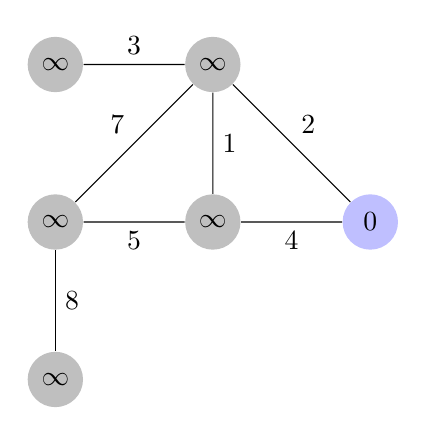
\begin{tikzpicture}[x=2cm, y=2cm]
            \tikzstyle{vertex}=[circle,fill=black!25,minimum size=20pt,inner sep=2pt]
            \tikzstyle{explored}=[circle,fill=green!25,minimum size=20pt,inner sep=2pt]
            \tikzstyle{current}=[circle,fill=blue!25,minimum size=20pt,inner sep=2pt]

            \node[vertex] (G_1) at (0,1)  {$\infty$};
            \node[vertex] (G_2) at (1,1)  {$\infty$};
            \node[current] (G_3) at (2,0)  {$0$};
            \node[vertex] (G_4) at (1,0)  {$\infty$};
            \node[vertex] (G_5) at (0,0)  {$\infty$};
            \node[vertex] (G_6) at (0,-1)  {$\infty$};

            \draw (G_1) -- (G_2) node[midway,above] {$3$} -- (G_3) node[midway,above right] {$2$}-- (G_4) node[midway,below] {$4$} -- (G_5) node[midway,below] {$5$} -- cycle;
            \draw (G_5) -- (G_2) node[midway,above left] {$7$} -- (G_4) node[midway,right] {$1$} -- cycle;
            \draw (G_5) -- (G_6) node[midway,right] {$8$} -- cycle;
        \end{tikzpicture}
    \end{center}
    Here, a blue node represents the node we are currently exploring and nodes that we have already explored will be drawn as green.
    \begin{center}
    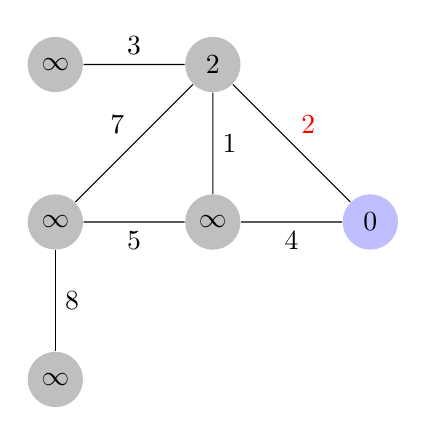
\begin{tikzpicture}[x=2cm, y=2cm]
        \tikzstyle{vertex}=[circle,fill=black!25,minimum size=20pt,inner sep=2pt]
        \tikzstyle{explored}=[circle,fill=green!25,minimum size=20pt,inner sep=2pt]
        \tikzstyle{current}=[circle,fill=blue!25,minimum size=20pt,inner sep=2pt]

        \node[vertex] (G_1) at (0,1)  {$\infty$};
        \node[vertex] (G_2) at (1,1)  {$2$};
        \node[current] (G_3) at (2,0)  {$0$};
        \node[vertex] (G_4) at (1,0)  {$\infty$};
        \node[vertex] (G_5) at (0,0)  {$\infty$};
        \node[vertex] (G_6) at (0,-1)  {$\infty$};

        \draw (G_1) -- (G_2) node[midway,above] {$3$} -- (G_3) node[midway,above right,red] {$2$}-- (G_4) node[midway,below] {$4$} -- (G_5) node[midway,below] {$5$} -- cycle;
        \draw (G_5) -- (G_2) node[midway,above left] {$7$} -- (G_4) node[midway,right] {$1$} -- cycle;
        \draw (G_5) -- (G_6) node[midway,right] {$8$} -- cycle;
    \end{tikzpicture}\hspace{2mm}
    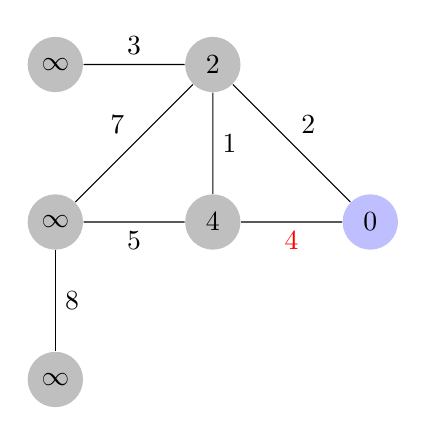
\begin{tikzpicture}[x=2cm, y=2cm]
        \tikzstyle{vertex}=[circle,fill=black!25,minimum size=20pt,inner sep=2pt]
        \tikzstyle{explored}=[circle,fill=green!25,minimum size=20pt,inner sep=2pt]
        \tikzstyle{current}=[circle,fill=blue!25,minimum size=20pt,inner sep=2pt]

        \node[vertex] (G_1) at (0,1)  {$\infty$};
        \node[vertex] (G_2) at (1,1)  {$2$};
        \node[current] (G_3) at (2,0)  {$0$};
        \node[vertex] (G_4) at (1,0)  {$4$};
        \node[vertex] (G_5) at (0,0)  {$\infty$};
        \node[vertex] (G_6) at (0,-1)  {$\infty$};

        \draw (G_1) -- (G_2) node[midway,above] {$3$} -- (G_3) node[midway,above right] {$2$}-- (G_4) node[midway,below,red] {$4$} -- (G_5) node[midway,below] {$5$} -- cycle;
        \draw (G_5) -- (G_2) node[midway,above left] {$7$} -- (G_4) node[midway,right] {$1$} -- cycle;
        \draw (G_5) -- (G_6) node[midway,right] {$8$} -- cycle;
    \end{tikzpicture}
    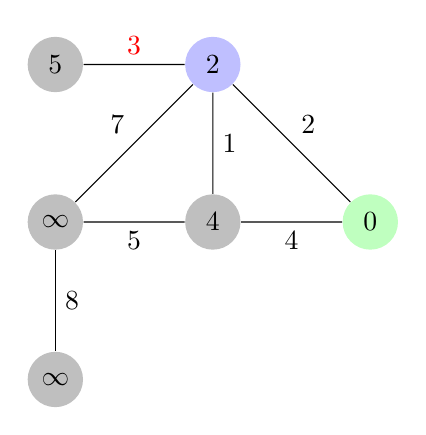
\begin{tikzpicture}[x=2cm, y=2cm]
        \tikzstyle{vertex}=[circle,fill=black!25,minimum size=20pt,inner sep=2pt]
        \tikzstyle{explored}=[circle,fill=green!25,minimum size=20pt,inner sep=2pt]
        \tikzstyle{current}=[circle,fill=blue!25,minimum size=20pt,inner sep=2pt]

        \node[vertex] (G_1) at (0,1)  {$5$};
        \node[current] (G_2) at (1,1)  {$2$};
        \node[explored] (G_3) at (2,0)  {$0$};
        \node[vertex] (G_4) at (1,0)  {$4$};
        \node[vertex] (G_5) at (0,0)  {$\infty$};
        \node[vertex] (G_6) at (0,-1)  {$\infty$};

        \draw (G_1) -- (G_2) node[midway,above,red] {$3$} -- (G_3) node[midway,above right] {$2$}-- (G_4) node[midway,below] {$4$} -- (G_5) node[midway,below] {$5$} -- cycle;
        \draw (G_5) -- (G_2) node[midway,above left] {$7$} -- (G_4) node[midway,right] {$1$} -- cycle;
        \draw (G_5) -- (G_6) node[midway,right] {$8$} -- cycle;
    \end{tikzpicture}
    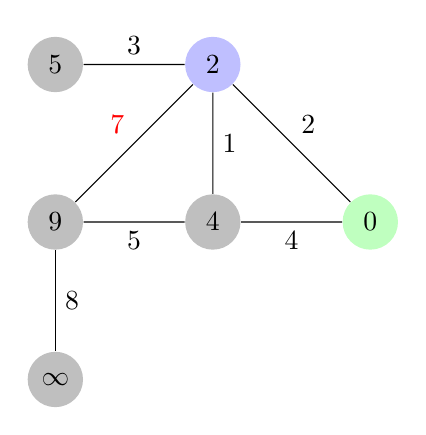
\begin{tikzpicture}[x=2cm, y=2cm]
        \tikzstyle{vertex}=[circle,fill=black!25,minimum size=20pt,inner sep=2pt]
        \tikzstyle{explored}=[circle,fill=green!25,minimum size=20pt,inner sep=2pt]
        \tikzstyle{current}=[circle,fill=blue!25,minimum size=20pt,inner sep=2pt]

        \node[vertex] (G_1) at (0,1)  {$5$};
        \node[current] (G_2) at (1,1)  {$2$};
        \node[explored] (G_3) at (2,0)  {$0$};
        \node[vertex] (G_4) at (1,0)  {$4$};
        \node[vertex] (G_5) at (0,0)  {$9$};
        \node[vertex] (G_6) at (0,-1)  {$\infty$};

        \draw (G_1) -- (G_2) node[midway,above] {$3$} -- (G_3) node[midway,above right] {$2$}-- (G_4) node[midway,below] {$4$} -- (G_5) node[midway,below] {$5$} -- cycle;
        \draw (G_5) -- (G_2) node[midway,above left,red] {$7$} -- (G_4) node[midway,right] {$1$} -- cycle;
        \draw (G_5) -- (G_6) node[midway,right] {$8$} -- cycle;
    \end{tikzpicture}
    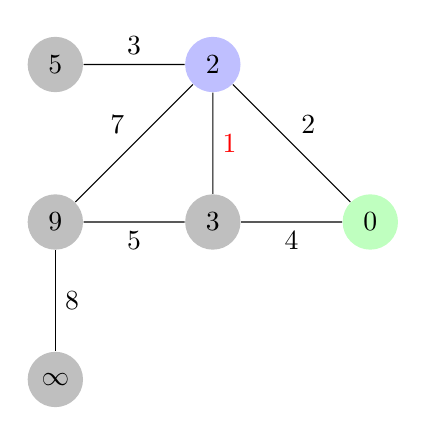
\begin{tikzpicture}[x=2cm, y=2cm]
        \tikzstyle{vertex}=[circle,fill=black!25,minimum size=20pt,inner sep=2pt]
        \tikzstyle{explored}=[circle,fill=green!25,minimum size=20pt,inner sep=2pt]
        \tikzstyle{current}=[circle,fill=blue!25,minimum size=20pt,inner sep=2pt]

        \node[vertex] (G_1) at (0,1)  {$5$};
        \node[current] (G_2) at (1,1)  {$2$};
        \node[explored] (G_3) at (2,0)  {$0$};
        \node[vertex] (G_4) at (1,0)  {$3$};
        \node[vertex] (G_5) at (0,0)  {$9$};
        \node[vertex] (G_6) at (0,-1)  {$\infty$};

        \draw (G_1) -- (G_2) node[midway,above] {$3$} -- (G_3) node[midway,above right] {$2$}-- (G_4) node[midway,below] {$4$} -- (G_5) node[midway,below] {$5$} -- cycle;
        \draw (G_5) -- (G_2) node[midway,above left] {$7$} -- (G_4) node[midway,right,red] {$1$} -- cycle;
        \draw (G_5) -- (G_6) node[midway,right] {$8$} -- cycle;
    \end{tikzpicture}
    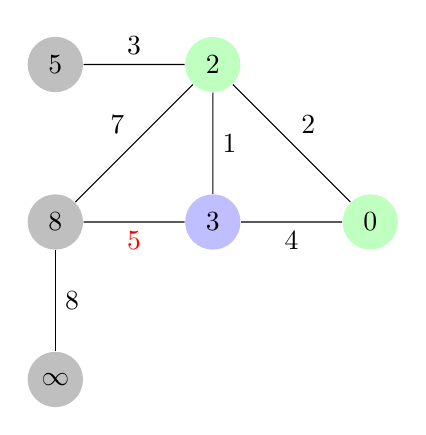
\begin{tikzpicture}[x=2cm, y=2cm]
        \tikzstyle{vertex}=[circle,fill=black!25,minimum size=20pt,inner sep=2pt]
        \tikzstyle{explored}=[circle,fill=green!25,minimum size=20pt,inner sep=2pt]
        \tikzstyle{current}=[circle,fill=blue!25,minimum size=20pt,inner sep=2pt]

        \node[vertex] (G_1) at (0,1)  {$5$};
        \node[explored] (G_2) at (1,1)  {$2$};
        \node[explored] (G_3) at (2,0)  {$0$};
        \node[current] (G_4) at (1,0)  {$3$};
        \node[vertex] (G_5) at (0,0)  {$8$};
        \node[vertex] (G_6) at (0,-1)  {$\infty$};

        \draw (G_1) -- (G_2) node[midway,above] {$3$} -- (G_3) node[midway,above right] {$2$}-- (G_4) node[midway,below] {$4$} -- (G_5) node[midway,below,red] {$5$} -- cycle;
        \draw (G_5) -- (G_2) node[midway,above left] {$7$} -- (G_4) node[midway,right] {$1$} -- cycle;
        \draw (G_5) -- (G_6) node[midway,right] {$8$} -- cycle;
    \end{tikzpicture}
    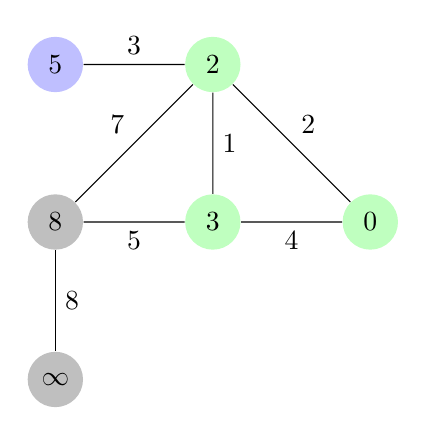
\begin{tikzpicture}[x=2cm, y=2cm]
        \tikzstyle{vertex}=[circle,fill=black!25,minimum size=20pt,inner sep=2pt]
        \tikzstyle{explored}=[circle,fill=green!25,minimum size=20pt,inner sep=2pt]
        \tikzstyle{current}=[circle,fill=blue!25,minimum size=20pt,inner sep=2pt]

        \node[current] (G_1) at (0,1)  {$5$};
        \node[explored] (G_2) at (1,1)  {$2$};
        \node[explored] (G_3) at (2,0)  {$0$};
        \node[explored] (G_4) at (1,0)  {$3$};
        \node[vertex] (G_5) at (0,0)  {$8$};
        \node[vertex] (G_6) at (0,-1)  {$\infty$};

        \draw (G_1) -- (G_2) node[midway,above] {$3$} -- (G_3) node[midway,above right] {$2$}-- (G_4) node[midway,below] {$4$} -- (G_5) node[midway,below] {$5$} -- cycle;
        \draw (G_5) -- (G_2) node[midway,above left] {$7$} -- (G_4) node[midway,right] {$1$} -- cycle;
        \draw (G_5) -- (G_6) node[midway,right] {$8$} -- cycle;
    \end{tikzpicture}
    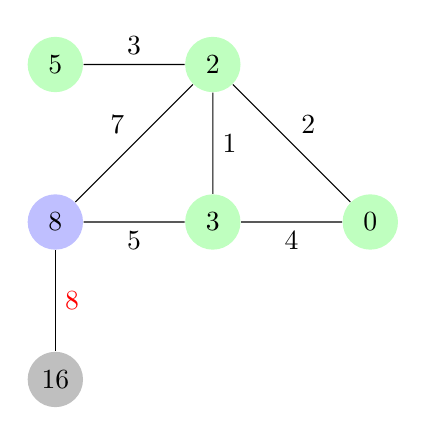
\begin{tikzpicture}[x=2cm, y=2cm]
        \tikzstyle{vertex}=[circle,fill=black!25,minimum size=20pt,inner sep=2pt]
        \tikzstyle{explored}=[circle,fill=green!25,minimum size=20pt,inner sep=2pt]
        \tikzstyle{current}=[circle,fill=blue!25,minimum size=20pt,inner sep=2pt]

        \node[explored] (G_1) at (0,1)  {$5$};
        \node[explored] (G_2) at (1,1)  {$2$};
        \node[explored] (G_3) at (2,0)  {$0$};
        \node[explored] (G_4) at (1,0)  {$3$};
        \node[current] (G_5) at (0,0)  {$8$};
        \node[vertex] (G_6) at (0,-1)  {$16$};

        \draw (G_1) -- (G_2) node[midway,above] {$3$} -- (G_3) node[midway,above right] {$2$}-- (G_4) node[midway,below] {$4$} -- (G_5) node[midway,below] {$5$} -- cycle;
        \draw (G_5) -- (G_2) node[midway,above left] {$7$} -- (G_4) node[midway,right] {$1$} -- cycle;
        \draw (G_5) -- (G_6) node[midway,right,red] {$8$} -- cycle;
    \end{tikzpicture}
    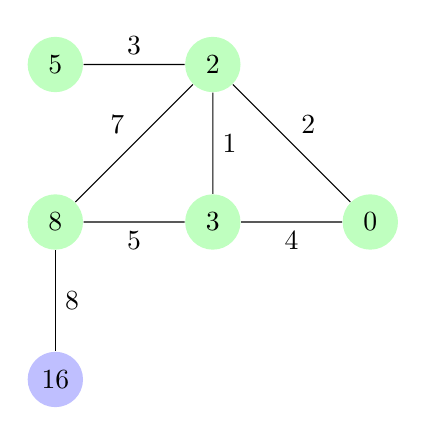
\begin{tikzpicture}[x=2cm, y=2cm]
        \tikzstyle{vertex}=[circle,fill=black!25,minimum size=20pt,inner sep=2pt]
        \tikzstyle{explored}=[circle,fill=green!25,minimum size=20pt,inner sep=2pt]
        \tikzstyle{current}=[circle,fill=blue!25,minimum size=20pt,inner sep=2pt]

        \node[explored] (G_1) at (0,1)  {$5$};
        \node[explored] (G_2) at (1,1)  {$2$};
        \node[explored] (G_3) at (2,0)  {$0$};
        \node[explored] (G_4) at (1,0)  {$3$};
        \node[explored] (G_5) at (0,0)  {$8$};
        \node[current] (G_6) at (0,-1)  {$16$};

        \draw (G_1) -- (G_2) node[midway,above] {$3$} -- (G_3) node[midway,above right] {$2$}-- (G_4) node[midway,below] {$4$} -- (G_5) node[midway,below] {$5$} -- cycle;
        \draw (G_5) -- (G_2) node[midway,above left] {$7$} -- (G_4) node[midway,right] {$1$} -- cycle;
        \draw (G_5) -- (G_6) node[midway,right] {$8$} -- cycle;
    \end{tikzpicture}
    \end{center}
    We can show this below via Python:
    \inputpython{dijkstra.py}{27}{67}
    To obtain the path, we can implement a dictionary \pyth{prev} and whenever the path to a certain node improves, we call: \pyth{prev[con["node"].name] = cur.name}.

    To add one vertex to $S$, we must search through all possible vertices so the runtime complexity is $\mathcal{O}(|V|^2)$.
    \subsection{Using Priority Queue}
    It is possible to improve the runtime to $\mathcal{O}(|E|\log |V|)$ using a priority queue:
    \inputpython{dijkstra.py}{71}{115}
    This algorithm is essentially the same, but instead of traversing explored nodes via BFS, we traverse it by sorting the nodes by their distance from the origin. The upper bound on the number of times a node is pushed is $2|E|$ and popping/pushing into \pyth{pq} has a time complexity of $\mathcal{O}(\log|V|)$. The time complexity of this algorithm is thus $\mathcal{O}(|E|\log|V|)$.
    \subsection{Greedy Best First Search}
    The general theme of search algorithms is to select a way to traverse explored nodes. In the simple method, it was via BFS. In the priority queue method, it was prioritizing nodes with a smaller distance. In the greedy best first search, it is by using a heuristic function $h(v)$ that gives a rough estimate of the distance between a node and the destination.

    For example, take the below graph and suppose we wish to move from \node{C} to \node{A}. Unlike the previous examples, the length of each path corresponds to their weights, so we can imagine these as physical points in space. We can let our heuristic function be the \textit{Manhattan distance} $\Delta x + \Delta y$:
    \begin{center}
        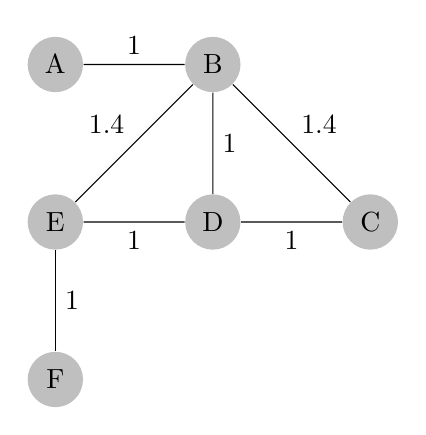
\begin{tikzpicture}[x=2cm, y=2cm]
            \tikzstyle{vertex}=[circle,fill=black!25,minimum size=20pt,inner sep=2pt]
            \node[vertex] (G_1) at (0,1)  {A};
            \node[vertex] (G_2) at (1,1)  {B};
            \node[vertex] (G_3) at (2,0)  {C};
            \node[vertex] (G_4) at (1,0)  {D};
            \node[vertex] (G_5) at (0,0)  {E};
            \node[vertex] (G_6) at (0,-1)  {F};

            \draw (G_1) -- (G_2) node[midway,above] {$1$} -- (G_3) node[midway,above right] {$1.4$}-- (G_4) node[midway,below] {$1$} -- (G_5) node[midway,below] {$1$} -- cycle;
            \draw (G_5) -- (G_2) node[midway,above left] {$1.4$} -- (G_4) node[midway,right] {$1$} -- cycle;
            \draw (G_5) -- (G_6) node[midway,right] {$1$} -- cycle;
        \end{tikzpicture}
    \end{center}
    We will start from \node{C} and look at the neighbours. The neighbour that minimizes the Manhattan distance is \node{B}, which directly leads to \node{A}. As you can expect, this is \textit{really bad}. It doesn't even bother checking if going to \node{D} is faster, but if we have a good heuristic, this isn't necessary. We can implement it in Python below:
    \inputpython{greedy.py}{1}{64}
    \subsection{A*}
    The A* algorithm is more robust, and combines the advantages of using a heuristic function with a priority queue. It is extremely similar to the optimized version of dijkstra's, except the priority queue is sorted by the heuristic function. We can also implement it in Python:
    \inputpython{A.py}{1}{60}
    
    \section{Trees}
    A \textit{tree} is a collection of nodes and directed edges. Here are some additional definitions not defined above:
    \begin{itemize}
        \item The \textbf{length} of a path is the number of edges it contains, not the number of nodes.
        \item For each node $n$, the \textbf{depth} of $n$ is the length of the unique path from the root to $n$.
        \item The \textbf{height} of $n$ is the length of the longest path from $n$ to a leaf.
        \item The height of a tree is equal to the height of the root node of a tree.
        \item The \textbf{branching factor} is the maximum number of children in any of its nodes.
        \item A \textbf{level} is the set of all nodes in the tree at a given depth.
        \item A \textbf{complete} tree is one where all levels are full except the bottom level, which has been filled from left to right.
        \item A \textbf{full tree} is a complete tree whose last level has been filled completely.
    \end{itemize}
    For example, consider the following graph:
    \begin{center}
    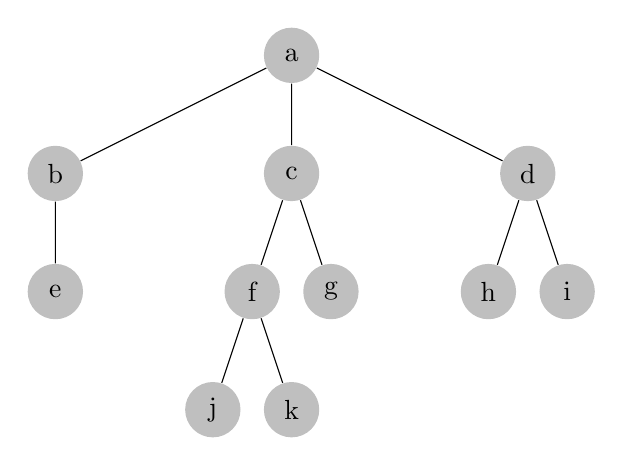
\begin{tikzpicture}[heap]
        \node {a}
        child{
            node{b}
            child{
                node{e}
            }
        }
        child{
            node{c}
            child{
                node{f}
                child{
                    node{j}
                }
                child{
                    node{k}
                }
            }
            child{
                node{g}
            }
        }
        child{
            node{d}
            child{
                node{h}
            }
            child{
                node{i}
            }
        }
        ;
      \end{tikzpicture}
    \end{center}
    A \textbf{binary tree} is a tree with a branching factor of $2$.
    \begin{itemize}
        \item The path $\node{c}\to \node{f}\to \node{k}$ has length $2$.
        \item The depth of \node{f} and the depth of \node{g} are both $2$.
        \item The height of \node{f} is $1$ and the height of \node{g} is $0$.
        \item The depth of \node{a} is $0$.
        \item The height of the tree is $3$. 
    \end{itemize}
    We will implement a tree from scratch, using Python. For simplicity, I will consider a binary tree (such that the same code can be used / expanded for future sections)
    \inputpython{tree.py}{1}{15}
    which represents (if you can't tell from the cleverly structured code) the graph:
    \begin{center}
    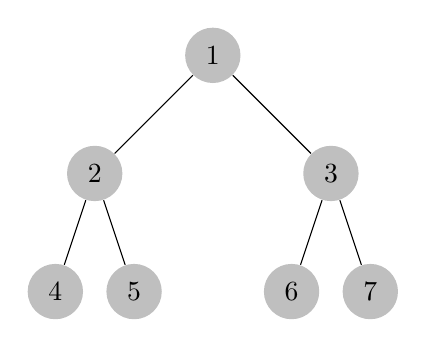
\begin{tikzpicture}[heap]
        \node {1}
        child{
            node{2}
            child{
                node{4}
            }
            child{
                node{5}
            }
        }
        child{
            node{3}
            child{
                node{6}
            }
            child{
                node{7}
            }
        }

        ;
      \end{tikzpicture}
    \end{center}
    \subsection{Traversal}
    Oftentimes, we wish to visit all the nodes in the tree in a particular order, and then apply some operation to each node. There are two types of traversal: preorder and postorder.
    
    For \textbf{preorder}, we perform an operation on the node first, then recursively do the same thing to its children. Suppose we wish to print out all the nodes. Then, we can write the function $\verb#pre_visualize#$
    \inputpython{tree.py}{17}{22}
    In the above example, we get the output: $\node{1}$, $\node{2}$, $\node{4}$, $\node{5}$, $\node{3}$, $\node{6}$, $\node{7}$. However, we can print the node \textit{after} we recursively call the function. This is what \textbf{postorder} does:
    \inputpython{tree.py}{26}{31}
    which outputs: $\node{4}$, $\node{5}$, $\node{2}$, $\node{6}$, $\node{7}$, $\node{3}$, $\node{1}$.
    
    Specifically for a binary tree, we can traverse it in \textbf{inorder}, where we perform the operation in between the recursive calls:
    \inputpython{tree.py}{35}{42}
    which outputs: $\node{4}$, $\node{2}$, $\node{5}$, $\node{1}$, $\node{6}$, $\node{3}$, $\node{7}$.

    \subsection{Binary Search Tree}
    If we want to find a node with a specific value in a random tree, the worst case scenario is $O(n)$. However, we can improve this by using a \textbf{binary search tree}. The conditions for a tree to be a binary search tree are:
    \begin{itemize}
        \item Must be a binary tree.
        \item All nodes in the left subtree of a node with value $k$ have a value less than $k$
        \item All nodes in the right subtree of a node with value $k$ have a value greater than $k$
    \end{itemize}
    This means that all values are different. For example, an example of a binary search tree (though not unique) would be:
    \begin{center}
        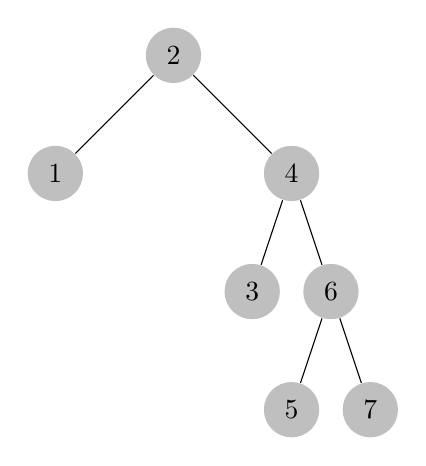
\begin{tikzpicture}[heap]
            \node{2}
            child{
                node{1}
            }
            child{
                node{4}
                child{
                    node{3}
                }
                child{
                    node{6}
                    child{
                        node{5}
                    }
                    child{
                        node{7}
                    }
                }
            }
    
            ;
        \end{tikzpicture}
    \end{center}
    which is represented below:
    \inputpython{tree.py}{46}{56}
    \subsection{Searching}
    We can search this tree recursively:
    \inputpython{tree.py}{58}{62}
    If the height is $h$, then the time complexity is $\mathcal{O}(h)$. However, the worst case scenario is still $\mathcal{O}(n)$. This is because $n=h$ is possible if we go from smallest to largest as we go from top to bottom.
    \subsubsection{Insertion}
    We can insert into a BST in a similar manner, where we traverse down, attempting to locate a certain value, and when we hit a null object, we insert it in that position. For example, in the below example, we insert \node{0} into our binary search tree:
    \inputpython{tree.py}{66}{79}
    \begin{idea}
        Here, the C implementation may be even cleaner with the help of pointers. To implement a tree, the children of each node aren't stored as ``objects,'' but instead they are stored as addresses. Therefore, all we need to do is recursively call $\verb#insert_BST#$ depending on whether the value is smaller or larger than each node, and when we hit the null pointer, we write in the desired node at that address. This approach \textit{does not work} in Python (to the best of my knowledge).
        \vspace{2mm}

        This general pattern will continue, though for AVL trees, we will implement it in \textit{C}.
    \end{idea}
    \subsubsection{Deletion}
    To delete a node, we again traverse the graph until we find the node we wish to delete. Unlike insertion, this isn't always a leaf node. Therefore, it is more complicated and there are three cases:
    \begin{itemize}
        \item \textbf{Case 1: No Children:} Easiest case. Simply remove it.
        \item \textbf{Case 2: One Child:} Replace the current node with the child.
        \item \textbf{Case 3: Two Children:} Do not delete the node. Instead, swap the node with its successor and delete the node from its new location.
    \end{itemize}
    The \textbf{successor} is the next larger value in the tree such that it is larger or equal to the left child, and smaller or equal to the right child. We can find the successor by finding the smallest value in the right subtree:
    \inputpython{tree.py}{83}{89}
    Here, we attempt to find the successor to $\node{4}$, which happens to be $\node{5}$. Using this, we can now implement deletion using the casework described above.
    \subsection{AVL Trees}
    AVL trees are a \textbf{balanced binary search tree}, with a \textit{balance condition}: For every node, the height of the left and right subtree differs by at most $1$. This is to ensure that we keep the height to be approximately $h \approx \log_2(n)$. The implementation is very similar to a regular binary search tree, except after inserting and deleting, we tweak the graph to balance it. For example, the following tree (that we saw above) is \textit{not} balanced:
    \begin{center}
        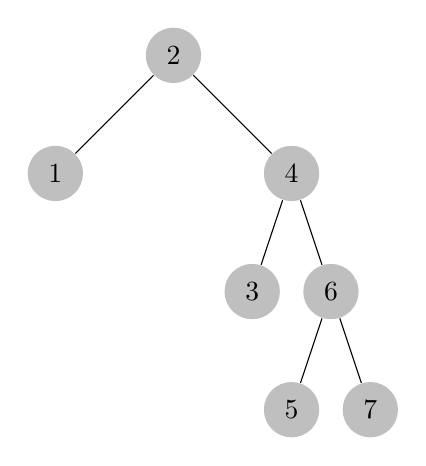
\begin{tikzpicture}[heap]
            \node{2}
            child{
                node{1}
            }
            child{
                node{4}
                child{
                    node{3}
                }
                child{
                    node{6}
                    child{
                        node{5}
                    }
                    child{
                        node{7}
                    }
                }
            }
    
            ;
        \end{tikzpicture}
    \end{center}
    \subsection{Balancing Outer Imbalances}
    For purposes of generalization, we will use $\tree{x}$ to represent a subtree. For example, the following is a graph where the left subtree of the left child is too high:
    \begin{center}
        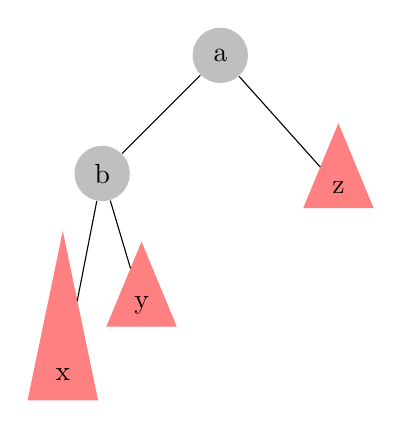
\begin{tikzpicture}[heap]
            \node{a}
            child{
                node{b}
                child{
                    node[big tree]{x}
                }
                child{
                    node[tree]{y}
                }
            }
            child{
                node[tree]{z}
            }
            ;
        \end{tikzpicture}
    \end{center}
    This can be fixed by performing a single rotation:
    \begin{center}
        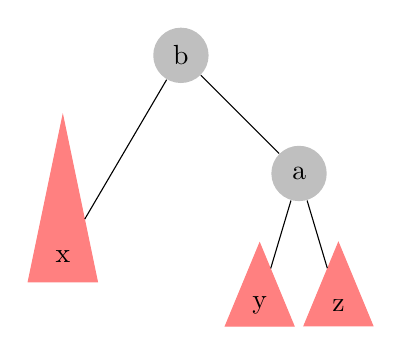
\begin{tikzpicture}[heap]
            \node{b}
            child{
                node[big tree]{x}
            }
            child{
                node{a}
                child{
                    node[tree]{y}
                }
                child{
                    node[tree]{z}
                }
            }
            ;
        \end{tikzpicture}
    \end{center}
    Notice that the BST property is still satisfied:
    \begin{itemize}
        \item $\tree{x}$ is still a left subtree of $\node{b}$.
        \item $\tree{y}$ is still in the right subtree of $\node{b}$.
        \item $\tree{z}$ is still in the right subtree of $\node{b}$.
        \item $b < a$, so $a$ can be a right child of $b$.
    \end{itemize}
    This is a \textbf{left rotation} that is quite simple to represent in programming. We simply have to write:
    \begin{python}
        a.left = b.right
        b.right = a
    \end{python}
    Similarly, we can also perform \textbf{right rotations}. Suppose, we have the graph:
    \begin{center}
        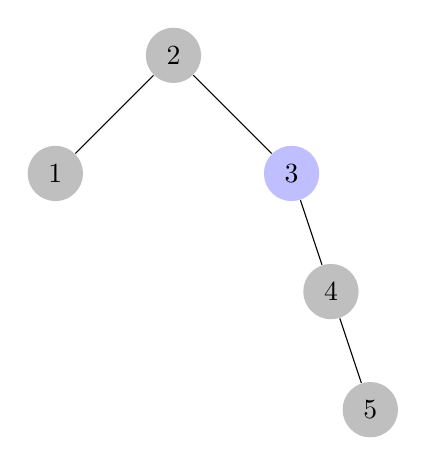
\begin{tikzpicture}[heap]
            \node{2}
            child{
                node{1}
            }
            child{
                node[fill=blue!25]{3}
                child[missing]{
                    node{}   
                }
                child{
                    node{4}
                    child[missing]{
                        node{}   
                    }
                    child{
                        node{5}
                    }
                }
            }
            ;
        \end{tikzpicture}
    \end{center}
    We can perform a right rotation on $\node{3}$ to turn the tree into:
    \begin{center}
        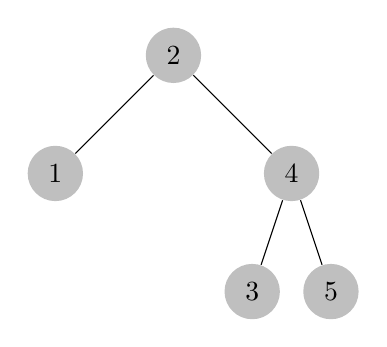
\begin{tikzpicture}[heap]
            \node{2}
            child{
                node{1}
            }
            child{
                node{4}
                child{
                    node{3}   
                }
                child{
                    node{5}
                }
            }
            ;
        \end{tikzpicture}
    \end{center}
    To be more precise, the above example is an \textbf{outside imbalance}, as the imbalance is caused in a subtree that is outside. This can be fixed using a single rotation.
    \subsection{Balancing Inner Imbalances}
    If the imbalance is not at the outside, we need to use more than one rotation. For example, if we tried to perform a single rotation on the graph to the left, we will end up with the graph to the right
    \begin{center}
        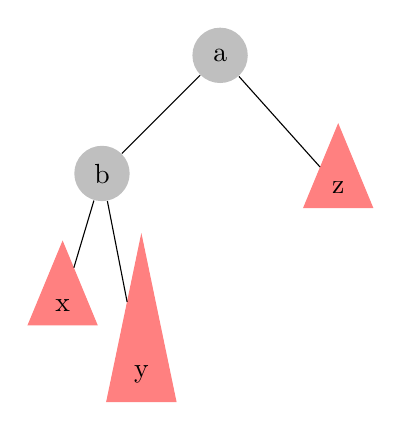
\begin{tikzpicture}[heap]
            \node{a}
            child{
                node{b}
                child{
                    node[tree]{x}
                }
                child{
                    node[big tree]{y}
                }
            }
            child{
                node[tree]{z}
            }
            ;
        \end{tikzpicture}
        \hspace{30mm}
        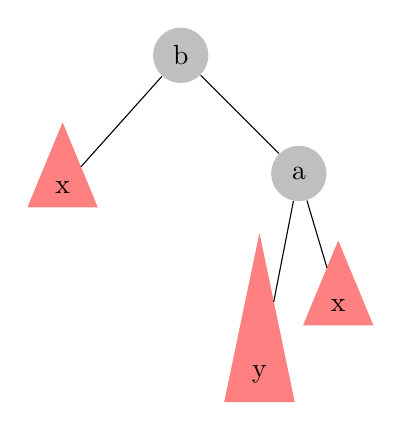
\begin{tikzpicture}[heap]
            \node{b}
            child{
                node[tree]{x}
            }
            child{
                node{a}
                child{
                    node[big tree]{y}
                }
                child{
                    node[tree]{x}
                }
            }
            ;
        \end{tikzpicture}
    \end{center}
    which is still not balanced! Instead, we have to expand our tree a bit and represent it as:
    \begin{center}
        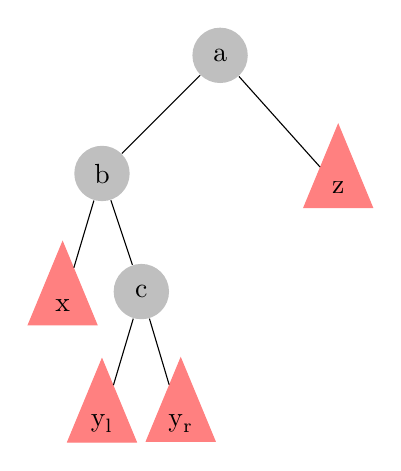
\begin{tikzpicture}[heap]
            \node{a}
            child{
                node{b}
                child{
                    node[tree]{x}
                }
                child{
                    node{c}
                    child{
                        node[tree]{$\text{y}_\text{l}$}
                    }
                    child{
                        node[tree]{$\text{y}_\text{r}$}
                    }
                }
            }
            child{
                node[tree]{z}
            }
            ;
        \end{tikzpicture}
    \end{center}
    We can balance this by rotating $\node{b}$ to the left (below left), then $\node{a}$ to the right (below right).
    \begin{center}
        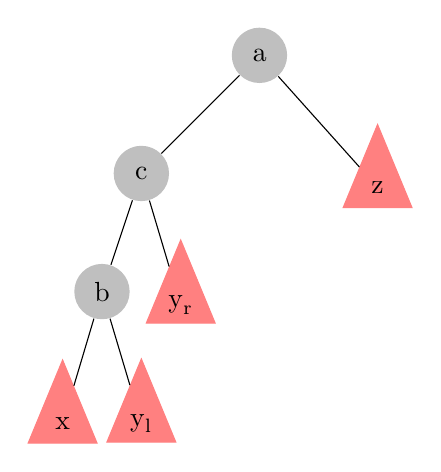
\begin{tikzpicture}[heap]
            \node{a}
            child{
                node{c}
                child{
                    node{b}
                    child{
                        node[tree]{x}
                    }
                    child{
                        node[tree]{$\text{y}_\text{l}$}
                    }
                }
                child{
                    node[tree]{$\text{y}_\text{r}$}
                }
            }
            child{
                node[tree]{z}
            }
            ;
        \end{tikzpicture}
        \hspace{30mm}
        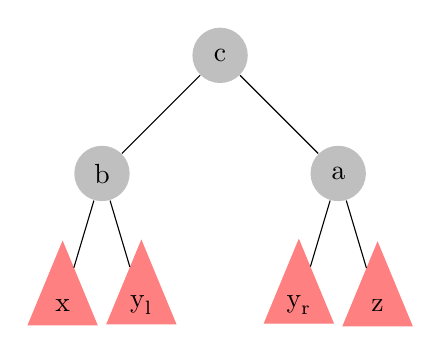
\begin{tikzpicture}[heap]
            \node{c}
            child{
                node{b}
                child{
                    node[tree]{x}
                }
                child{
                    node[tree]{$\text{y}_\text{l}$}
                }
            }
            child{
                node{a}
                child{
                    node[tree]{$\text{y}_\text{r}$}
                }
                child{
                    node[tree]{z}
                }
            }
            ;
        \end{tikzpicture}
    \end{center}
    While this may seem complicated, it is not too difficult to implement:
    \begin{python}
        c.left = b
        c.right = a
        b.right = root(yl)
        a.left = root(yr)
    \end{python}
    Implementation of AVL trees using \textit{C} is provided on the course website. Make sure to be familiar with how the code works.
    \section{Hashing}
    A \textbf{map} is a collection of $\verb#(key, value)#$ pairs. The keys are unique, but the values may not be. This is equivalent to a \textit{Python} dictionary. There are two main operations:
    \begin{itemize}
        \item $\verb#get(key)#$ returns the value corresponding to a given key.
        \item $\verb#put(key, value)#$ creates a new instance of a key and value pair.
    \end{itemize}
    Our motivation is to increase the time efficiency of $\verb#get(key)#$ as much as possible. There are a few methods:
    \begin{itemize}
        \item Store the keys in an unsorted array: The efficiency is $\mathcal{O}(n)$.
        \item Store the keys in an AVL tree (or something similar). The efficiency is $\mathcal{O}(n)$.
        \item Store the values in an array, where the index \textit{is} the key. The efficiency is $\mathcal{O}(1)$.
    \end{itemize}
    While this last method may sound superior, it may take up a lot of space as keys can be spread apart a lot, and there is a lot of memory allocated that isn't used. The idea of hashing is to implement this same idea, but only using a table size of $n$.
    \vspace{2mm}

    We can define the hashing function to be:
    \begin{equation}
        h(x) = x \% n
    \end{equation}
    Here, $x$ is the key\footnote{This implies that the key must be an integer. If it was a string, we can convert it into an integer using the ASCII value of the characters, and perform similar things for other types.} and $\%$ gives the remainder once $x$ is divided by $n$. It is possible to combine hash functions, say if the key is a compound object:
    \begin{equation}
        h(s,x) = (h(s)p_1 + h(x)p_2) \% n
    \end{equation}
    where $p_1$ and $p_2$ are relatively prime (we don't want to factor the expression)
    \subsection{Collisions}
    The problem with this hashing function is that it is not a bijection. For example, if $n=10$, then the key $13$ and $23$ would represent the same point in memory.
    
    \subsubsection{Chaining}
    We can solve this by using a linked list. For example, if we try to put the key $23$ in memory (i.e. index $3$) and there is already a linked list defined there (even if it contains only one key), then we just attach the desired key to the end of the linked list.

    The runtime depends on the number of elements in a list on average. The \textbf{load factor} $\lambda$ represents the average number of elements stored in each table entry:
    \begin{equation}
        \lambda = \frac{k}{\text{table size}}
    \end{equation}
    where $k$ is the number of entries. If lookup fails (key is not in the hash table), we need to search on average $\lambda$ nodes. If lookup succeeds, we need to search on average $\lambda/2+1$ nodes. We want to keep $\lambda \approx 1$ and we can do this by increasing the table size as needed.
    \subsubsection{Probing}
    Instead of storing a linked list at each entry, we can store just the key-value pair. If a collision occurs, we put the pair in an empty cell of the hash table instead. In \textbf{linear probing}, we empty cell we put it in is the \textit{next empty cell}. During probing, the load factor is always smaller or equal to $\lambda \le 1$. The table is full if $\lambda = 1$. In general, if there is a collision, we want to put our key-value pair in the index:
    \begin{equation}
        (h(x)+f(i))\% n
    \end{equation}
    where $i=1,2,3,\dots$. The type of probing depends on $f$:
    \begin{itemize}
        \item Linear Probing: Try the next cell: $f(i)=i$.
        \begin{itemize}
            \item The biggest problem is \textit{primary clustering}. Full cells tend to cluster with no free cells in between. The time required to find an empty cell can become very large if the table is almost full (i.e. if $\lambda \approx 1$)
        \end{itemize}
        \item Quadratic Probing: $f(i)=i^2$.
        \begin{itemize}
            \item Although primary clustering is no longer a prob lem, if the table gets too full (i.e. $\lambda > 0.5$), then it is possible that certain cells become unreachable.
            \begin{theorem}
                The \textbf{Quadratic Problem Theorem}: If $n$ is prime, then the first $n/2$ cells visited by quadratic probing are distinct. Therefore, it's always possible to find an empty cell if the table is at most half full.
                \begin{proof}
                    Suppose there is a repetition. Then:
                    \begin{equation}
                        (h+i^2) \% n = (h+j^2) \% n
                    \end{equation}
                    Therefore:
                    \begin{equation}
                        h+i^2 = h + j^2 + kn
                    \end{equation}
                    for some integer $n$. We can factor this to be:
                    \begin{equation}
                        kn = (i+j)(i-j)
                    \end{equation}
                    Since $n$ is prime, either $i+j$ or $i-j$ must be divisible by $T$. But since $i<j<n$, both $i-j$ and $i+j$ are too small.
                \end{proof}
            \end{theorem}
        \end{itemize}
        \item Double Hashing: $f(i) = i h_2(x)$
        \begin{itemize}
            \item Do not worry too much about this.
        \end{itemize}
    \end{itemize}
    \newpage
    \section{Neural Networks}
    \subsection{Overview}
    Machine Learning is in a nutshell, is just a graph theory problem. It takes in a series of inputs $x_i$ (i.e. pixels in an image), and through a series of linear transformations, creates the outputs $z_i$ (i.e. probability an image is Justin Bieber)
    \begin{center}
        \begin{neuralnetwork}[height=3, nodesize=30pt, layerspacing=35mm, nodespacing=15mm, layertitleheight=5em]
            \newcommand{\x}[2]{$x_#2$}
            \newcommand{\y}[2]{$z_#2$}
            \newcommand{\hfirst}[2]{\small $h^{(1)}_#2$}

            \inputlayer[count=3, bias=false, title=Input\\layer, text=\x]
            \hiddenlayer[count=4, bias=false, title=Hidden\\layer, text=\hfirst,] \linklayers
            \outputlayer[count=3, title=Output\\layer, text=\y] \linklayers
        \end{neuralnetwork} 
    \end{center}
    Intuitively, the hidden layers act as templates. For example, if $x_i$ represent pixels, then $h^{(1)}_i$ can represent combinations of pixels (i.e. lines) and if we have another hidden layer, that can represent combinations of lines (i.e. shapes). Each arrow represents a certain weight, which corresponds to how important a particular node is for the template we're looking for.
    
    Many of this is still traditional programming. The important thing about neural networks is that there can be thousands of nodes, and the weights are determined by the computer, not manually inputted by humans. This means that the computer will ``learn'' to recognize lines and shapes as setting these particular weights provides the highest rate of success.

    In \textbf{supervised machine learning}, we train the neural network by providing it with a test set, where $z_i$ is known. It then tries to minimize the error by shifting the weights. This shifting of weights is the mechanism we will be exploring.
    
    The value of each node of interest is given by:
    \begin{equation}
        \sum (w_{(j,i)} h_i) + b_j
    \end{equation}
    where $h_i$ is the value of the node before it, $w_{(j,i)}$ is the weight of the connection, and $b_j$ is the bias of the node of interest.
    \begin{warning}
        To be more rigorous, we can write each weight as:
        \begin{equation}
            W^{(h,j,i)}
        \end{equation}
        where $h$ refers to the layer, $i$ refers to node in that layer, and $j$ refers to the node in the previous layer given by the connection. However, for our purposes, I chose to leave out this notation so I can focus on the concepts, not the syntax.
    \end{warning}
    \subsection{Activation Function}
    Each node can theoretically take a value from $-\infty$ to $\infty$, and we don't want one particularly high node to dominate. As a result, we normalize all values to between $0$ and $1$, using the activation function:
    \begin{equation}
        \sigma(t) = \frac{1}{1+\exp(-t)}
    \end{equation}
    which graphically, looks like this:
    \begin{center}
        \begin{tikzpicture}
        \begin{axis}[
        title=Activation Function,
        axis lines = box,
        xlabel = $t$,
        ylabel = $y$,
        variable = t,
        trig format plots = rad,
        ]
        \addplot [
            domain=-10:10,
            samples=70,
            color=blue,
            ]
            {1/(1+e^(-t))};
        \addlegendentry{$\sigma(t)$}
        
        \end{axis}
        \end{tikzpicture}
    \end{center}
    \subsection{Cost Function}
    A common cost function (we encountered this in ESC103) is the least square error. If $o$ is the prediction, and $y$ is the actual result, then we can let the cost be:
    \begin{equation}
        C(o,y) = \sum_{i=1}^m \left|y_i - o_i \right|^2
    \end{equation}
    Note that for larger datasets, we may have to pass in data as batches, and the cost would be the average cost of each batch.
    \subsection{Gradient Descent}
    Let $W$ be a vector representing the weights. Then we want to set the new weight $W_\text{new}$ to be:
    \begin{equation}
        W_\text{new} = W - \alpha \nabla_W C(o,y) = W - \alpha \begin{bmatrix}
            f_{w_1}C \\ f_{w_2}C \\ \vdots 
        \end{bmatrix}
    \end{equation}
    and the biases to be:
    \begin{equation}
        B_\text{new} = B - \alpha \nabla_B C(o,y)
    \end{equation}
    The partial derivative of $C$ with respect to $w_{(j,i)}$ is given by:
    \begin{align}
        \frac{\partial C}{\partial w_{(j,i)}} &= \frac{\partial o}{\partial w_{(j,i)}} \frac{\partial C}{\partial o}
    \end{align}
    Letting $o_i = \sigma\left(\sum w_{(j,i)}h_j + b_i\right)$, we can use the chain rule to get:
    \begin{align}
        \frac{\partial C}{\partial w_{(j,i)}} &= \frac{\partial (\sum w_{(j,i)}h_j)}{\partial w_{(j,i)}}\frac{\partial \sigma}{\partial (\sum w_{(j,i)}h_j)}\frac{\partial C}{\partial o} \\ 
        &= h_j \frac{\partial \sigma}{\partial(\sum w_{(j,i)}h_j)}\frac{\partial C}{\partial o} \\ 
        &= h_j \sigma'\left(\sum_{j} w_{(j,i)}h_j + b_i\right) \frac{\partial}{\partial o_i}C
    \end{align}
    Note that:
    \begin{equation}
        \sigma'(t) = \sigma(t)(1-\sigma(t))
    \end{equation}
    and:
    \begin{equation}
        \frac{\partial C}{\partial o_i} \sum_{i=1}^N (o_i-y_i)^2 = 2(o_i - y_i)
    \end{equation}
    we can simplify this to:
    \begin{equation}
        \boxed{
            \frac{\partial C}{\partial w_{(j,i)}} = 
            2h_j o_i (1-o_i) (o_i - y_i)
        }
    \end{equation}
    To re-iterate, $w_{(j,i)}$ refers to a certain weight between two nodes, $h_j$ refers to the previous node, $o_i$ refers to the node of interest, and $y_i$ refers to the desired value. Since we can only have desired values for the output nodes, this equation \textit{only} describes how the cost function changes with respect to how weights connected to the output nodes changes.

    However, we can generalize this to other nodes using the chain rule:
    \begin{equation}
        \frac{\partial C}{\partial w_{(1,j,i)}}
    = \frac{\partial C}{\partial h_i} \frac{\partial h_i}{\partial w_{(1,j,i)}}
    \end{equation}
    Here:
    \begin{equation}
        \frac{\partial C}{\partial h_i} = \sum_k \frac{\partial C}{\partial o_k}\frac{\partial o_k}{\partial h_i}
    \end{equation}
    \begin{idea}
        This really isn't too difficult, it's just the notation is hard to understand. Write out equations for the network, and apply ESC195 knowledge. To do so, we make use of an example:
    \end{idea}
    \subsection{A Quick Example:}
    Suppose we have the graph:
    \begin{center}
        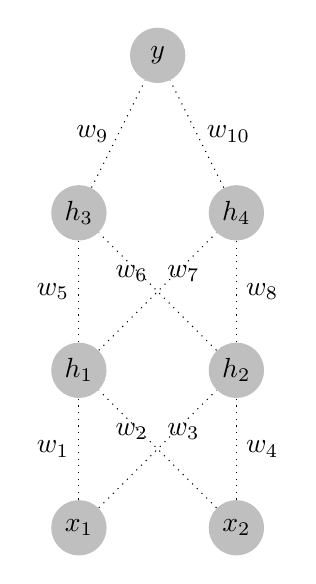
\begin{tikzpicture}[x=1cm, y=1cm]
            \tikzstyle{vertex}=[circle,fill=black!25,minimum size=20pt,inner sep=2pt]
            \node[vertex] (y)  at (1,6)  {$y$};
            \node[vertex] (h1) at (0,2)  {$h_1$};
            \node[vertex] (h2) at (2,2)  {$h_2$};
            \node[vertex] (h3) at (0,4)  {$h_3$};
            \node[vertex] (h4) at (2,4)  {$h_4$};
            \node[vertex] (x1) at (0,0)  {$x_1$};
            \node[vertex] (x2) at (2,0)  {$x_2$};

            \draw[dotted] (x1) -- (h2) node[midway, above right] {$w_3$};
            \draw[dotted] (x2) -- (h1) node[midway, above left] {$w_2$};
            \draw[dotted] (x1) -- (h1) node[midway, left] {$w_1$};
            \draw[dotted] (x2) -- (h2) node[midway, right] {$w_4$};

            \draw[dotted] (h1) -- (h4) node[midway, above right] {$w_7$};
            \draw[dotted] (h2) -- (h3) node[midway, above left] {$w_6$};
            \draw[dotted] (h1) -- (h3) node[midway, left] {$w_5$};
            \draw[dotted] (h2) -- (h4) node[midway, right] {$w_8$};

            \draw[dotted] (h3) -- (y)  node[midway,left] {$w_9$};
            \draw[dotted] (h4) -- (y)  node[midway,right] {$w_{10}$};
        \end{tikzpicture}
    \end{center}
    To calculate $\frac{\partial C}{\partial w_{10}}$, we have:
    \begin{equation}
        \frac{\partial C}{\partial w_9} = \frac{\partial C}{\partial y}\frac{\partial y}{\partial w_{10}}
    \end{equation}
    From earlier, we have:
    \begin{equation}
        \frac{\partial y}{\partial w_{10}} = h_4y(1-y) 
    \end{equation}
    To calculate $\frac{\partial C}{\partial w_1}$, we have:
    \begin{equation}
        \frac{\partial C}{\partial w_1} = \frac{\partial C}{\partial y}\frac{\partial y}{\partial h_3}\frac{\partial h_3}{\partial h_1}\frac{\partial h_1}{\partial w_1} + \frac{\partial C}{\partial y}\frac{\partial y}{\partial h_4}\frac{\partial h_4}{\partial h_1}\frac{\partial h_1}{\partial w_1}
    \end{equation}
    This chain of partial derivatives can be made more clear by drawing a ``chain rule tree,'' similar to what is done in Stewart. Each path corresponds to a different term in the sum. For the above example, we would draw:
    \begin{center}
        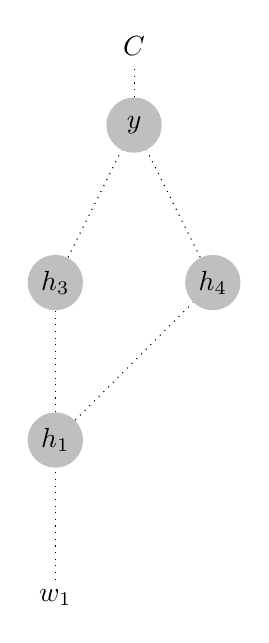
\begin{tikzpicture}[x=1cm, y=1cm]
            \tikzstyle{vertex}=[circle,fill=black!25,minimum size=20pt,inner sep=2pt]
            \node (C)  at (1,7)  {$C$};
            \node[vertex] (y)  at (1,6)  {$y$};
            \node[vertex] (h1) at (0,2)  {$h_1$};
            \node[vertex] (h3) at (0,4)  {$h_3$};
            \node[vertex] (h4) at (2,4)  {$h_4$};
            \node (x1) at (0,0)  {$w_1$};

            \draw[dotted] (x1) -- (h1);

            \draw[dotted] (h1) -- (h4);
            \draw[dotted] (h1) -- (h3);

            \draw[dotted] (h3) -- (y);
            \draw[dotted] (h4) -- (y);

            \draw[dotted] (y) -- (C);
        \end{tikzpicture}
    \end{center}
    Again, note that:
    \begin{equation}
        \frac{\partial h_1}{\partial w_1} = x_1h_1(1-h_1)
    \end{equation}
    and:
    \begin{equation}
        \frac{\partial h_3}{\partial h_1} = w_5h_3(1-h_3)
    \end{equation}
    and we can do similar computations for the other partial derivatives.
\end{document}
